%% LaTeX2e class for student theses
%% thesis.tex
%% 
%% Karlsruhe Institute of Technology
%% Institute for Program Structures and Data Organization
%% Chair for Software Design and Quality (SDQ)
%%
%% Dr.-Ing. Erik Burger
%% burger@kit.edu
%%
%% Version 1.3.2, 2017-08-01

%% Available page modes: oneside, twoside
%% Available languages: english, ngerman
%% Available modes: draft, final (see README)
\documentclass[twoside, english]{sdqthesis}
\usepackage{mathtools}
\usepackage{pgfplots}
\pgfplotsset
{
	compat                   = newest,
	every tick/.append style = thin,
	width= .95 \textwidth
}
% safe mode so we dont redefine \: etc
\usepackage[safe]{tipa}

%% ---------------------------------
%% | Information about the thesis  |
%% ---------------------------------

%% Name of the author
\author{Emanuel Jöbstl}

%% Title (and possibly subtitle) of the thesis
\title{Reverberation robust acoustic modelling using time delay neural networks}

%% Type of the thesis 
\thesistype{Master's Thesis}

%% Change the institute here, ``IPD'' is default
\myinstitute{Interactive Systems Lab}

%% You can put a logo in the ``logos'' directory and include it here
%% instead of the SDQ logo
% \grouplogo{myfile}
%% Alternatively, you can disable the group logo
% TODO: Put the CMU logo in the logos directory, remove nogrouplogo
\nogrouplogo

%% The reviewers are the professors that grade your thesis
\reviewerone{Prof. A}
\reviewertwo{Prof. B}

%% The advisors are PhDs or Postdocs
\advisorone{M.Sc. C}
%% The second advisor can be omitted
\advisortwo{M.Sc. D}

%% Please enter the start end end time of your thesis
\editingtime{4. November 2017}{4. May 2018}

\settitle

%% --------------------------------
%% | Settings for word separation |
%% --------------------------------

%% Describe separation hints here.
%% For more details, see 
%% http://en.wikibooks.org/wiki/LaTeX/Text_Formatting#Hyphenation
\hyphenation{
% me-ta-mo-del
}

%% --------------------------------
%% | Bibliography                 |
%% --------------------------------

%% Use biber instead of BibTeX, see README
\usepackage[citestyle=numeric,style=numeric,backend=biber]{biblatex}
\addbibresource{thesis.bib}

%% ====================================
%% ====================================
%% ||                                ||
%% || Beginning of the main document ||
%% ||                                ||
%% ====================================
%% ====================================
\begin{document}
\tikzset{%
	every neuron/.style={
		circle,
		draw,
		minimum size=1cm
	},	
	tdnn neuron/.style={
		rectangle,
		draw=black,
		fill=black!10,
		minimum height=0.5cm,
		minimum width=0.1cm 
	},
	neuron vmissing/.style={
		draw=none, 
		scale=4,
		text height=0.333cm,
		execute at begin node=\color{black}$\vdots$
	},
	neuron hmissing/.style={
		draw=none, 
		scale=2,
		text height=0.333cm,
		execute at begin node=\color{black}$\hdots$
	},
}

\tikzstyle{state}=[shape=circle,draw=black]
\tikzstyle{observation}=[shape=rectangle,draw=black]
\tikzstyle{lightedge}=[<-,dotted]
\tikzstyle{mainstate}=[state,thick]
\tikzstyle{mainedge}=[<-,thick]

\newcommand{\weightillustration}[3]{
\begin{minipage}{\linewidth}
	\centering
	\vspace{5mm}	
	\includegraphics[angle=90,width=0.9\linewidth]{#1}
	\captionof{figure}{#2}
	\label{#3}
\end{minipage}
}

\newcommand{\smallweightillustration}[3]{
	\begin{minipage}{\linewidth}
		\centering
		\vspace{5mm}	
		\includegraphics[angle=90,width=0.5\linewidth]{#1}
		\captionof{figure}{#2}
		\label{#3}
	\end{minipage}
}

%% Set PDF metadata
\setpdf

%% Set the title
\maketitle

%% The Preamble begins here
\frontmatter

\input{sections/declaration.tex}

\setcounter{page}{1}
\pagenumbering{roman}

%% ----------------
%% |   Abstract   |
%% ----------------
 
%% For theses written in English, an abstract both in English
%% and German is mandatory.
%%
%% For theses written in German, a German abstract is sufficient.
%%
%% The text is included from the following files:
%% - sections/abstract

\includeabstract

%% ------------------------
%% |   Table of Contents  |
%% ------------------------
\tableofcontents

\listoffigures
\listoftables

%% -----------------
%% |   Main part   |
%% -----------------

\mainmatter

%%% LaTeX2e class for student theses
%% sections/content.tex
%% 
%% Karlsruhe Institute of Technology
%% Institute for Program Structures and Data Organization
%% Chair for Software Design and Quality (SDQ)
%%
%% Dr.-Ing. Erik Burger
%% burger@kit.edu
%%
%% Version 1.3.2, 2017-08-01

\chapter{Introduction}
\label{ch:Introduction}

Automated Speech Recognition is an important way of human computer interaction. The fundamental problem Automated Speech Recognition attempts to solve is to transform natural spoken language to text, which can then easily be processed by computer systems. Especially with the advent of smart mobile devices, more and more use cases for Automated Speech Recognition are available, mainly in the form of smart assistants as described in \cite{lopez2017alexa}. There are also many use cases which are not facing end users, for example the automated transcription of university lectures, as outlined in \cite{muller2016lecture}.

Despite the recent success of automated speech recognition, many systems still rely on microphones which are close to the speaker, or microphone arrays and beam forming. For many use cases, this is a serious draw back. Users might want to use their smart assistant without picking up their device every time. During lectures, it is hard to transcribe questions from the audience. 

\cite{yoshioka2012making} gives a good overview about the problems that arise when distant microphones are used. The most prominent problem is reverberation. Reverberation happens, informally speaking, when a signal is interfered by weaker, delayed copies of itself. 

The goal of this work is to investigate how Automated Speech Recognition could be made more robust against reverberation. More specifically, a the focus is put on providing a more robust acoustic model using Time Delay Neural Networks. 

\section{Reverberation and reverberated Audio}

This section will focus on a formal definition of reverberation and provide some intuition why reverberation makes Automated Speech Recognition difficult. First, we give a very brief introduction to signal processing and system theory, according to the book \cite{leon2015signale}.

\subsection{Continuous Signals and Systems}

An audio signal can, as any other continuous \textit{signal}, be described as a continous function $y(t)$ where $t$ indicates the time. In literature, the argument $t$ is often dropped  when not explicitly needed to make equations easier to read.  
Signals can be fed into \textit{systems}, which in turn creates an output signal. In the context of this work, we only consider linear, time invariant systems. 
\\
Let $S$ be a linear time invariant system, $y_1$, $y_2$ continuous signals, and $c_1$, $c_2$ constants. The following properties hold if and only if a given system is an linear time invariant system: 

\[S\{c_1 y_1(t) + c_2 y_2(t)\} = c_1 S\{y_1(t)\} + c_2 S\{y_2(t)\} \tag{linearity}\]

The linear property allows us to treat application of a system to a signal as a linear transformation in the function space our signals are defined in. 

\[y_1(t) = S\{y_2(t)\} \implies y_1(t - t0) = S\{y_2(t - t0)\} \tag{time invariance}\]

The time invariance property guarantees that the behavior of a system never depends on the time. In other words, if the input signal to a system is shifted in time, the only difference to the output is a shift in time as well.

\[
\begin{rcases*}
y_1(t') = y_2(t') \\
x_1(t') = S\{y_1(t')\} \\ 
x_2(t') = S\{y_2(t')\} \\
\end{rcases*} \implies x_1(t') = x_2(t') \tag{causality}\]

The causality property guarantees that, if two signals are equal for all times $t'$ before a chosen time $t_0$, the output signals of the system processing this signals will also be equal up to this point. Simply put, the output of a system up to time $t_0$ can not depend on any input that happens after $t_0$. It is worth to note that all real systems are always causal. 
\\ \\
A linear time-invariant system can be characterized by its so called impulse response $g$, defined as the system output when presented with a so called dirac impulse $\delta$.

\[g(t) = S\{\delta(t)\}\]

The dirac impulse $\delta$ is a function that is formally defined by the following equation. 

\begin{align}
g(t_2) = \int_{-\infty}^{\infty} y(t)\delta(t - t_2) dt \label{eq:dirac} 
\end{align}

It can be said that the dirac impulse is zero for all $t$ not equal to zero. The integral over the dirac impulse defined to be one. 
\\ \\
Given definition \ref{eq:dirac}, as well as the linear property, we can show that the impulse response of a system is indeed sufficient to calculate the output signal for any given input signal. 
\begin{align*}
x(t) &= S\{y(t)\} \\
	 &= S\left\{\int_{-\infty}^{\infty} y(\tau)\delta(\tau - t) d\tau \right\} \\
	 &= \int_{-\infty}^{\infty} y(\tau)S\{\delta(\tau - t)\} d\tau \\
	 &= \int_{-\infty}^{\infty} y(\tau)g(\tau - t) d\tau
\end{align*}

Furthermore, we define the convolution operation, $*$, for two given signals as follows.

\[
 (y_1 * y_2)(t) = \int_{-\infty}^{\infty} y(\tau)y_2(\tau - t) d\tau \tag{(convolution)}
\]

A convolution is thus an operation that combines two functions to create a new function. Given this definition, we can write the output signal $x$ of a system $S$ given an input signal $y$ as convolution with the impulse response $g$ of the system. 

\[
x(t) = S\{y(t)\} = (y * g)(t)
\]

\subsection{Properties of Reverberation}

The acoustic properties of a room can be approximated as a linear time invariant system. The properties of this system are dependent on the properties of the room itself, for example the shape, size and surface of the wall, as well as the location of the sound source and the location of the receiver. Especially regarding automated speech recognition, \cite{ritter2016training} gives results that show that the location of a speaker relative to the microphone can have a very large impact on recognition results.

The measured impulse response of a real reverberation can be seen in figure \ref{fig:air_rir}. This specific sample is taken from the Aachen Impulse Response database \cite{jeub2009binaural}. Such a sample can be created by creating a very brief sound impulse, for example a clap, in an otherwise silent room, and then recording the sound for a few seconds. 

As described in \cite{yoshioka2012making}, we can divide the impulse response into the direct sound itself, early reflections, and late reverberation. The intuition behind is that the original sound wave arrives at the receiver first. After that, reflections of the signal which were reflected once by the walls of the room arrive. These reflections are already dampened significantly. Then, reflections of reflections will be received, and so on, until the sound waves become so weak that the room is silent again. 
\\ \\
\begin{minipage}{\linewidth}
	\makebox[\linewidth]{
		\begin{tikzpicture}
			\begin{axis}[ytick=\empty,height=6cm, ylabel=Amplitude, xlabel=Milliseconds, 
			xticklabel style={name=T\ticknum}]
			\addplot table [x expr=\coordindex / 4,y=amplitude,color=black,mark=none] {data/air0053bilecture};
			
			\end{axis}	
			\draw[] (1.2,4) -- (1,4) node[anchor=east,font=\tiny] {Sound};
			\draw[decorate, decoration={brace}] (1.3,3.2) -- (3.00,3.2) node[midway, anchor=south,font=\tiny] {Early Reflections};	
			\draw[decorate, decoration={brace}] (3.05,3.2) -- (11.8,3.2) node[midway, anchor=south,font=\tiny] {Late Reverberations};
		\end{tikzpicture}
	}	
	\captionof{figure}{Room impulse response of a lecture hall}
	\label{fig:air_rir}
\end{minipage}

It is important to note that late reverberations can be measurable for several hundred milliseconds.\\\\

To illustrate the impact of reflection and reverberation in a more formal way, we can use the decomposition into direct sound, early reflection, and late reverberation. We define a rather crude approximation of a room impulse response that subsequently overlays an audio signal with weaker copies of itself.

\[
g_{rir}(t) = w_0 \delta(t) + \sum_{1}^{n} w_n * \delta(t - t_n)
\]

Here, $w_n$ are weighting factors, which represent the dampening of our reflections. $t_n$ are the delays until our reflection is received. We now consider the system $S_{rir}$ associated with the impulse response $g_{rir}$, apply the audio signal $y$ and observe the output $x$.

\begin{align*}
x(t) &= S_{rir}\{y(t)\} \\
     &= (g_{rir} * y)(t) \\
     &= \int_{-\infty}^{\infty} g(\tau)y(\tau - t) d\tau \\
     &= \int_{-\infty}^{\infty} \left[ w_0 \delta(t) + \sum_{n} w_n * \delta(t - t_n)\right] y(\tau - t) d\tau \\
     &= \int_{-\infty}^{\infty} \delta(t) y(\tau - t) d\tau + \sum_{n}  \int_{-\infty}^{\infty} w_n \delta(t - t_n) y(\tau - t) d\tau  \\
     &= w_0 y(t) + \sum_{n} w_n y(t - t_n)
\end{align*}

If the room impulse response is non-zero over at a certain time interval $t_n$, the audio signal produced at $t$ will still influence the received signal $x$ at $t + t_n$. 

\subsection{Impact of Reverberation on Digital Audio Samples}

Before formally introducing automated speech recognition during a later chapter, we want to show that the impact of reverberation can be significant for many applications that process sound or speech.\\ \\
Before a signal can be processed on a computer, it has to be measured. This process is called \textit{sampling}. Formally, we can describe sampling as the following operation, where $t_A$ is called the sampling interval. We call $y_{digital}$ a discrete signal. 

\[
y_{digital}(t) = y(t) * \sum_{n = 0}^{\infty} \delta{t - nt_A} 
\]

Since this yields a time series of infinite length, signals are usually cut into pieces, which are then independently processed from each other. This is called windowing. For the most simple form of windowing, we can set all signal values outside of a certain range to be zero. Formally, this can be defined by multiplying the signal with a rectangle function $\sigma_{rect,a}(t)$ .

\[
\sigma_{rect,a}(t) = \begin{cases}
1 &,-a < t < a \\
0
\end{cases}
\]

When working with signals, especially for classification tasks, methods built upon the \textit{fourier transform} are used very often. The fourier transform transforms a signal $y(t)$ from its time domain to the frequency domain $Y(f)$. The resulting function $Y(f)$ is called the spectrum and gives the distribution of energy over all frequencies for the original signal $y(t)$. The fourier transformation can be defined for continuous or discrete signals, as well as for discrete and windowed signals. In the case of discrete and windowed signal, this is called the \textit{short time fourier transform}, which was first described in \cite{gabor1946theory}. It can formally be defined as follows, with an arbitrary window function $\sigma$:

\[
Y(n, \omega) = \sum_{m = -\infty}^{\infty} y(mt_A) \sigma((n - m)t_A) e^{-j \omega n}  
\]

The function $Y(n, \omega)$ gives the signal magnitude for a certain time window $n$ and a frequency window $\omega$. The time resolution depends reciprocally on the frequency resolution and vice versa. It is not possible to increase the frequency resolution while not decreasing the time resolution.\\ \\

We can investigate the effects of a reverberated signal on the short time fourier transform by applying the same approach as in the previous chapter. The resulting short time fourier spectrum of the reverberated and sampled signal is given as follows.

\begin{align*}
Y(n, \omega) = \sum_{m = -\infty}^{\infty} w_0 y(mt_A) \sigma((n - m)t_A) e^{-j \omega n} + 
\sum_{m = -\infty}^{\infty} \sum_{n} w_n y(mt_A - t_n) \sigma((n - m)t_A) e^{-j \omega n}  
\label{eq:stftnoise}
\end{align*}

Equation \ref{eq:stftnoise} shows that, for sufficiently large $t_n$ and $w_n$, significant noise is added to neighboring time windows. To recapitulate from the last chapter, the $t_n$ for a large room can be up to several tenths of seconds, while the window size for most applications is in the hundreds of milliseconds. 
\\ \\
This mathematic observation shall serve as a motivation for this work. Reverberation, especially late reverberation can be a hard problem that significantly distorts measurements of signals. To cope with reverberation, our application has to consider large time windows in the first place. Time delay neural networks, which will be introduced in section \ref{ch:TDNN} can naturally deal with a such wide windows in a stable way. Before we explain the properties of time delay neural networks in depth, we first introduce neural networks in section \ref{sec:neural_networks} as well as the basics of automated speech recognition in section \ref{ch:HMM_ASR}. In chapter \ref{ch:approach} we will explain our solution in detail and then show experimental results in chapter \ref{ch:results}.
\\ \\
We conclude the introduction with a more visual example. Figure \ref{fig:air_spectrogram} shows the magnitude of the short term fourier transformation for a short speech segment, as well as the short term fourier transformation for the same speech segment after it has been reverberated using the impulse response shown in Figure \ref{fig:air_rir}. Such a magnitude representation is also called \textit{spectrogram} in literature. 


\begin{minipage}{\linewidth}
	\makebox[\linewidth]{
		\begin{tikzpicture}
		\begin{axis}[xlabel=Time, ylabel=Frequency, ytick=\empty, width= .50\textwidth, axis line style={draw=none}, axis x line*=bottom]
		\addplot [] 
		graphics[xmin=0,xmax=3,ymin=0,ymax=1] {images/abc_spectrogram.png};
		\end{axis}
		\end{tikzpicture}
		\begin{tikzpicture}
		\begin{axis}[xlabel=Time, ylabel=\empty, ytick=\empty, width= .50\textwidth, axis line style={draw=none}, axis x line*=bottom]
		\addplot [] 
		graphics[xmin=0,xmax=3,ymin=0,ymax=1] {images/abc_noise_spectrogram.png};
		\end{axis}
		\end{tikzpicture}
	}
	\captionof{figure}{Spectrogram of a clean and a reverberated audio sample. The left side shows a clean recording of a speaker saying \textit{``A B C''}. The right side shows the the recording after it was reverberated by the impulse response shown in Figure \ref{fig:air_rir}. It can clearly be seen that the reverberation caused the signal to become smudged along the time axis.}
	\label{fig:air_spectrogram}
\end{minipage}

%
\chapter{Related Work}

This chapter will give a brief introduction to neural networks and time delay neural networks, as well as an introduction automated speech recognition with hidden Markov models. These are the necessary building blocks for the work presented in this thesis. At the end of this chapter, we will also briefly present research that directly inspired this work. 

\section{Neural Networks}

In machine learning research, the goal of a \textit{neural network} is to approximate arbitrary functions. The basic idea of neural networks, so called \textit{perceptrons}, were first introduced by Rosenblatt in \cite{rosenblatt1958perceptron}. While the first neural networks were biologically motivated, neural networks can be interpreted as composition of functions. The relation between these functions forms a directed graph. In this work, we will only cover \textit{feed forward neural networks}. They are called feed forward neural networks because there are no feedback connections: The relation between all functions in the neural network forms an acyclic directed graph. Feed forward networks are an important building block for many machine learning applications. 
\\
More formally, as described in \cite{Goodfellow-et-al-2016}, a feed forward neural network can be described as a model $y = f^*(x, \theta)$, approximating an existing function $y = f(x)$. In this example $x$ is the input, $y$ is the output and $\theta$ are the model parameters which are learned during training. $f$ is the function to approximate and $f^*$ is a composition of many functions with the parameters $\theta$. 
\\
In practice, the functions composing a feed forward neural network are often simply chained, so that their relation graph simply forms a path. In this case, the functional components are called layers. A feed forward neural network of this form with $n$ layers can be written as follows:

\[y = f^*_n \dots (f^*_2(f^*_1(x, \theta_1), \theta_2) \dots, \theta_n)\]

For this type of neural network, $f^*_1$ is applied to the input, then $f^*_2$ is applied to the output of $f^*_1$, until the final layer is reached. The output of the final layer is the output of the neural network.

\begin{minipage}{\linewidth}
	\makebox[\linewidth]{
	\begin{tikzpicture}[x=1.5cm, y=1.5cm, >=stealth]
	
	
	%% TODO: How do we draw the arrows here? 
	\foreach \m/\l [count=\y] in {x,1,2,missing,n,y}
	\node [every neuron/.try, neuron \m/.try] (n\m) at (\y*1-1,2.5-0) {};
	%%\draw [->] (n\m) -- (n\lastm);
	
	\foreach \m/\l [count=\y] in {x,1,2,missing,n,y}
	
	\foreach \m/\l [count=\y] in {1,2,3,missing,4}
	\node [every neuron/.try, neuron \m/.try] (input-\m) at (0,2.5-\y) {};
	
	\foreach \m [count=\y] in {1,missing,2}
	\node [every neuron/.try, neuron \m/.try ] (hidden-\m) at (2,2-\y*1.25) {};
	
	\foreach \m [count=\y] in {1,missing,2}
	\node [every neuron/.try, neuron \m/.try ] (output-\m) at (4,1.5-\y) {};
	
	\foreach \l [count=\i] in {1,2,3,n}
	\draw [<-] (input-\i) -- ++(-1,0)
	node [above, midway] {$I_\l$};
	
	\foreach \l [count=\i] in {1,n}
	\node [above] at (hidden-\i.north) {$H_\l$};
	
	\foreach \l [count=\i] in {1,n}
	\draw [->] (output-\i) -- ++(1,0)
	node [above, midway] {$O_\l$};
	
	\foreach \i in {1,...,4}
	\foreach \j in {1,...,2}
	\draw [->] (input-\i) -- (hidden-\j);
	
	\foreach \i in {1,...,2}
	\foreach \j in {1,...,2}
	\draw [->] (hidden-\i) -- (output-\j);
	
	\foreach \l [count=\x from 0] in {Input, Hidden, Ouput}
	\node [align=center, above] at (\x*2,2) {\l \\ layer};
	
	\end{tikzpicture}
	}
\end{minipage}


Even with this simplification, it has been shown that such a feed forward neural network can approximate any function with any desired accuracy. This is called the \textit{universal approximation theorem}, the proof can be found in \cite{hornik1989multilayer}. The caveat is finding the correct function $f^*_n$ to use in each layer and the correct parameters $\theta_n$. Also, finding the function to approximate is non-trivial in the first place. We will discuss these problems in the next sections. 

\subsection{}



\label{ch:realted_work}
\subsection{ASR with HMM-based systems}
\label{ch:HMM_ASR}

This chapter will be focused on how ASR is done with Janus. It will contain: 
\begin{itemize}
	\item A brief introduction to HMM models
	\item A brief introduction to HMM-based ASR tools:
	\begin{itemize}
		\item description of n-gram language models, dictionaries and context-dependent phone models
		\item description of the purpose of an acoustic model
		\item explanation, about how the this component are combined to form a speech recognizer 
		\item example, showing how the language and phone models, as well as the dictionary are combined to form a HMM
	\end{itemize}
	\item A description of the Word-Error-Rate and Frame-Error-Rate metric. 
	\item An explanation about training HMM-based systems using the expected maximisation algorithm. 
\end{itemize}

\subsection{Time Delay Neural Networks}
\label{ch:TDNN}
The goal of this chaper is to provide a short introduction to neural networks, 
as well as explain the concept of TDNNs. It will contain:
\begin{itemize}
	\item A brief intro to MLPs and SGD
	\item Parameter coupling (convolutional neural networks)
	\item Time delay neural networks
	\item Interpretation of TDNNs as FIR filters
\end{itemize}

\subsection{Acoustic Modelling using Neural Networks}
\label{ch:acoustic_modelling}
The goal of this chapter is to describe the approach of using DNNs for acoustic modelling.
The contents will be: 
\begin{itemize}
	\item definition of the acoustic model training as a deep learning problem
	\item different discriminative training strategies
	\begin{itemize}
		\item Binary Cross Entropy loss on existing labels
		\item Bianry Cross Entropy with re-generating the labels, then trianing again
		\item Minimum Bayes Risk and variants, especially State-Minimum-Bayes-Risk
	\end{itemize}
	\item A brief section about common tricks used when trianing DNN acoustic models, 
	especially Exponential Decay/Newbob.
	\item If there is time left: A brief analysis of the 2nd derivative of the loss function
	during gradient descend.
\end{itemize}

\begin{minipage}{\linewidth}
	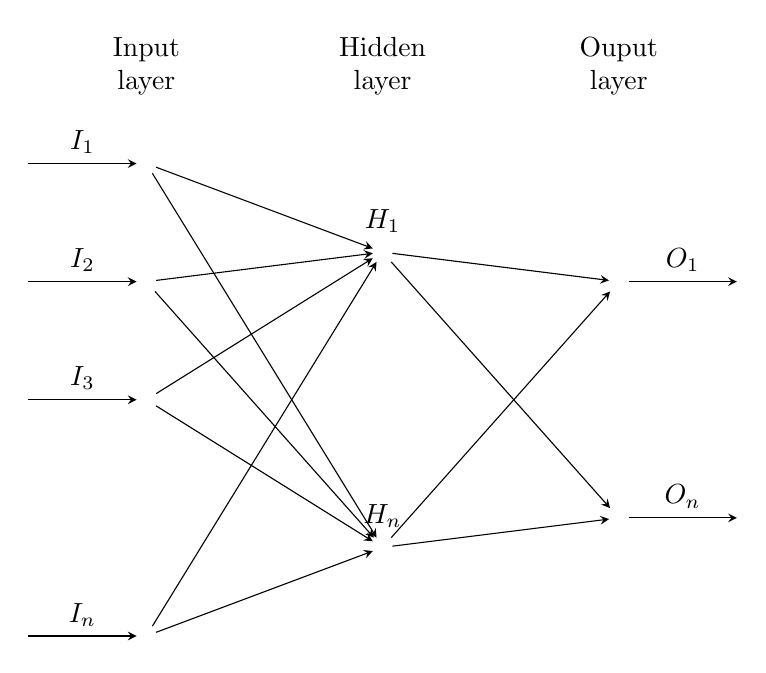
\begin{tikzpicture}[x=1.5cm, y=1.5cm, >=stealth]
	
	\foreach \m/\l [count=\y] in {1,2,3,missing,4}
	\node [every neuron/.try, neuron \m/.try] (input-\m) at (0,2.5-\y) {};
	
	\foreach \m [count=\y] in {1,missing,2}
	\node [every neuron/.try, neuron \m/.try ] (hidden-\m) at (2,2-\y*1.25) {};
	
	\foreach \m [count=\y] in {1,missing,2}
	\node [every neuron/.try, neuron \m/.try ] (output-\m) at (4,1.5-\y) {};
	
	\foreach \l [count=\i] in {1,2,3,n}
	\draw [<-] (input-\i) -- ++(-1,0)
	node [above, midway] {$I_\l$};
	
	\foreach \l [count=\i] in {1,n}
	\node [above] at (hidden-\i.north) {$H_\l$};
	
	\foreach \l [count=\i] in {1,n}
	\draw [->] (output-\i) -- ++(1,0)
	node [above, midway] {$O_\l$};
	
	\foreach \i in {1,...,4}
	\foreach \j in {1,...,2}
	\draw [->] (input-\i) -- (hidden-\j);
	
	\foreach \i in {1,...,2}
	\foreach \j in {1,...,2}
	\draw [->] (hidden-\i) -- (output-\j);
	
	\foreach \l [count=\x from 0] in {Input, Hidden, Ouput}
	\node [align=center, above] at (\x*2,2) {\l \\ layer};
	
	\end{tikzpicture}
\end{minipage}


\subsection{Acoustic Modelling using TDNNs.} 
%% LaTeX2e class for student theses
%% sections/content.tex
%% 
%% Karlsruhe Institute of Technology
%% Institute for Program Structures and Data Organization
%% Chair for Software Design and Quality (SDQ)
%%
%% Dr.-Ing. Erik Burger
%% burger@kit.edu
%%
%% Version 1.3.2, 2017-08-01



\chapter{Design of a TDNN acoustic model}
To find a good design for a TDNN acoustics model, we had to make several design decisions. Most of the design decisions were justified by experiments, while some were taken from related work. This chapter summarizes the decisions made and the corresponding results. In some cases, we will also provide a comparison with a fully-connected network, which served as our experiment baseline. It should be noted that the experiments described in \cite{peddinti2015jhu} and \cite{peddinti2015reverberation} provided the main inspiration for this work, therefore we based some of our parameters on their result. 

\subsection{Neural Network Parameters}
This section focuses on parameters that are related to the neural network design. 
\subsubsection{Input Context and Features}
The input context of all our TDNN models is ${-13,9}$, which means the TDNN sees the current frame, thirteen frames in the past, and nine frames in the future. This parameter was taken from the smallest TDNN model described in \cite{peddinti2015reverberation}. 
\subsubsection{Count and Width of Layers}
The count of layers and width of each layer is one of the most important design parameters for neural networks. As in \cite{peddinti2015reverberation}, all our models use the same amount of channels for each TDNN unit. Only the count of observed time frames changes with each layer. \\ \\
\begin{minipage}{\linewidth}
	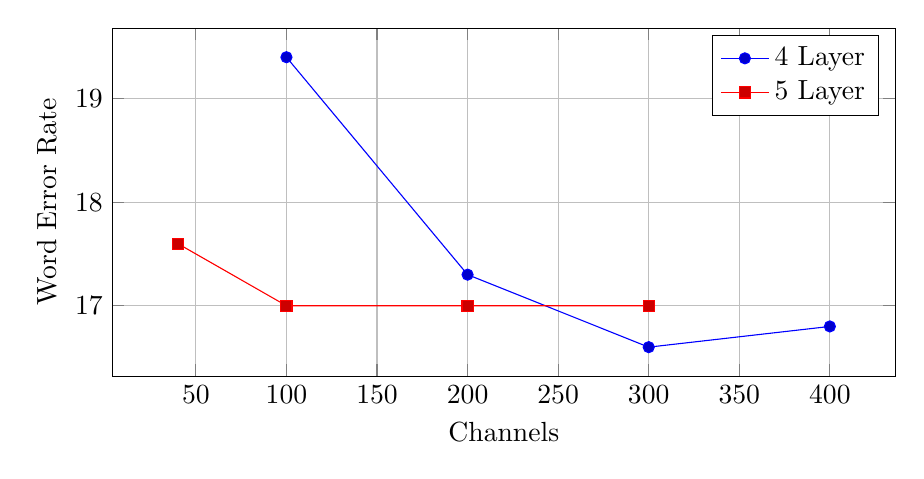
\begin{tikzpicture}
	\begin{axis}[ylabel=Word Error Rate, xlabel=Channels, height=6cm, 
	xticklabel style={name=T\ticknum},grid=major]
	\addplot coordinates {
		(100,19.4) %994
		(200,17.3) %999
		(300,16.6) %1009
		(400,16.8) %1010
	};
	\addlegendentry{4 Layer};
	\addplot coordinates {
		(40,17.6) %1040
		(100,17.0) %i3
		(200,17.0) %1039
		(300,17.0) %1036
	};
	\addlegendentry{5 Layer};
	\end{axis}
	\end{tikzpicture}
	\captionof{figure}{Word Error Rate for different choices of layer and channel count}
	\label{fig:tdnn_layer_design}
\end{minipage}
Figure \ref{fig:tdnn_layer_design} shows the word error rate for different configurations. The word error rate was estimated by using the same decoding parameters $l_p$ and $l_z$ for each architecture and the priors were estimated from the training data. Table \ref{tbl:tdnn_layer_design} gives the kernel size and stride over time for each layer in each architecture. \\ \\
\begin{minipage}{\linewidth}
	\centering 
	\begin{tabular} {|l | c | c | c | c | c | c | c | c | c | c | c | c |}
	\hline
	Model & \multicolumn{4}{c|}{4 Layer} & \multicolumn{5}{c|}{5 Layer} \\
	\hline
	Layer & 1 & 2 & 3 & 4 & 1 & 2 & 3 & 4 & 5 \\
	\hline
	Kernel Size & 5 & 2 & 2 & 2 & 5 & 5 & 3 & 2 & 2 \\
	\hline
	Stride & 3 & 2 & 2 & 2 & 2 & 1 & 1 & 1 & 1 \\
	\hline
	\end{tabular}
	\captionof{figure}{Splice and stride parameters for the two different architectures}
	\label{tbl:tdnn_layer_design}
\end{minipage}
For this set of experiments, each TDNN layer was followed by a LP-pooling nonlinearity with P of two and group size ten, as well as a batch normalization layer. 
\subsubsection{Nonlinearity}
Following\cite{zhang2014improving}, we use a LP-pooling nonlinearity with a P of two and a group size if ten after each TDNN layer. Using the LP norm can be problematic, as the gradient can become infinity when all inputs in the pooling group are zero. The authors of \cite{peddinti2015reverberation} propose to use a normalization layer after each LP-pooling layer, which solves the problem. We propose an alternate approach, which is setting the gradient to zero if all inputs become zero. Furthermore, we also tested max pooling as a possible nonlinearity. All experiments were conducted on the 4-Layer architecture described before. Figure \ref{fig:tdnn_nonlinearity} shows the results. 
\begin{minipage}{\linewidth}
	\begin{tikzpicture}
		\begin{axis}[
			   ybar,
			enlargelimits=0.15,
			legend style={at={(0.5,-0.2)},
				anchor=north,legend columns=-1},
			ylabel={\#participants},
			symbolic x coords={LP Batch Norm,MaxPool,LP Gradient Modification}
			%symbolic x coords={LP Batch Norm,MaxPool,LP Gradient Modificatoin},
			xtick=data,
			nodes near coords
		]
		
		% TODO: Fix this plot...
		\addplot coordinates {(LP Batch Norm,16.6) (MaxPool,15.8) 
			(LP Gradient Modification,15.5)};
	%	\addplot coordinates {1,16.6) (2,15.8) (3, 15.5)};
		%\addplot coordinates {(1,15.8)};
		%\addplot coordinates {(1,15.5)};
		
		%\legend{LP + Batch Norm, MaxPool, LP + Gradient Modification}
		\end{axis}
	\end{tikzpicture}
	\captionof{figure}{Word Error Rate for different choices of nonlinearities}
	\label{fig:tdnn_nonlinearity}
\end{minipage}
In our case, the usage of LP tuning with a modified gradient outperformed the other nonlinearities.  
\subsection{Training Parameters}

\subsection{Decoding Parameters}



\label{ch:approach}
This chapter describes our approach for acoustic modelling using TDNNs on a high level. 
We will also give a brief overview over unknown hyperparemters and design decisions,
as well as a coarse overview over the structure of our implementation. 

\chapter{Experiment Setup}
\label{ch:experiment_setup}
This chapter should describe the detailed preleminaries and hyperparemters of our training and evaluation setup:
\begin{itemize}
    \item which data, and which preprocessing was used
    \item how was the data reverbed
    \item which learning rate schedulers, optimizers, loss functions were used
    \item which mechanisms were used to make the training faster and scalable
\end{itemize}
%% LaTeX2e class for student theses
%% sections/evaluation.tex
%% 
%% Karlsruhe Institute of Technology
%% Institute for Program Structures and Data Organization
%% Chair for Software Design and Quality (SDQ)
%%
%% Dr.-Ing. Erik Burger
%% burger@kit.edu
%%
%% Version 1.3.2, 2017-08-01

\chapter{Evaluation on Reverberated Data}
\label{ch:results}
This section contains the final evaluation. It describes how our model compared to a fully connected baseline model performed. The baseline model was tested with different input contexts. The purpose is to rule out that our model performed better only because of the size of the input context. The speech recognition system and preprocessing used for this evaluation is described in detail in chapter \ref{ch:tdnn_design}.
\section{Neural Network Models}
We compare the final TDNN model with a fully connected baseline model that was also used in \cite{nguyen20162016}. This section describes these two models. 
\subsection{Fully Connected Baseline Model}
We compare the results of our TDNN with a fully connected network that achieved comparable performance on the development set. The model consists of six linear layers with a width of 1600, followed by ReLU nonlinearities. The output layer is a linear layer followed by a softmax nonlinearity. We tested input contexts of $(-13, 9)$ as well as $(-5, 5)$.
\subsection{TDNN Model}
The TDNN model, which can be seen in figure \ref{fig:final_tdnn}, is based on the results documented in chapter~\ref{ch:tdnn_design}. We tuned the hyperparameters so that the word error rate was minimal on the development set. \\ 

The model consists of four TDNN layers and one linear layer at the end, followed by a softmax nonlinearity. After each TDNN layer, a L2 pooling nonlinearity with a pool size of ten is used. As described in section \ref{sec:tdnn_nonlin}, we set the gradient to zero if all inputs to the L2 pooling layer are zero. A splicing layer with the splicing configuration $(0, 1, 2, 3, 3, 4, 5, 6)$ is inserted after the first TDNN layer. The exact configuration of kernel sizes and strides can be found in table \ref{tbl:tdnn_layer_design}. The output of each TDNN layer has 3000 channels, the output of each pooling layer has 300 channels. The input context is $(-13, 9)$. The count of channels, the modified L2 pooling gradient and the omission of batch normalization was the main difference to the architecture described in \cite{peddinti2015reverberation} and \cite{peddinti2015jhu}. 
\begin{minipage}{\linewidth}
	\vspace{5mm}
	\begin{tikzpicture}[x=1.8cm, y=1.5cm]
	% Input layer
	\node[text width=3cm] at (-1,0) {Input ($23\times40$)};
	\foreach \m in {2,3,...,22}
	\node [tdnn neuron] (input-\m) at (\m*0.25,0) {};
	
	\node [tdnn neuron, label=below:$x_{t - 13}$] (input-1) at (1*0.25,0) {};
	\node [tdnn neuron, label=below:$x_{t + 9}$] (input-23) at (23*0.25,0) {};
	
	% TDNN 1
	\node[text width=3cm] at (-1,0.5) {TDNN/L2 pool};
	\node[text width=3cm] at (-1,1) {Hidden ($7\times300$)};
	\foreach \m [count=\y] in {1,2,...,7}
	\node [tdnn neuron] (hidden-1-\m) at (\y*0.25*3,1) {};
	
	% Splice
	\node[text width=3cm] at (-1,1.5) {Splice};
	\node[text width=3cm] at (-1,2) {Hidden ($8\times300$)};
	\foreach \m [count=\y] in {1,2,...,8}
	\node [tdnn neuron] (hidden-2-\m) at (\y*0.25*3 - 0.40,2) {};
	
	% TDNN 2
	\node[text width=3cm] at (-1,2.5) {TDNN/L2 pool};
	\node[text width=3cm] at (-1,3) {Hidden ($4\times300$)};
	\foreach \m [count=\y] in {1,2,...,4}
	\node [tdnn neuron] (hidden-3-\m) at (\y*0.25*6 - 0.80,3) {};
	
	% TDNN 3
	\node[text width=3cm] at (-1,3.5) {TDNN/L2 pool};
	\node[text width=3cm] at (-1,4) {Hidden ($2\times300$)};
	\foreach \m [count=\y] in {1,2}
	\node [tdnn neuron] (hidden-4-\m) at (\y*0.25*12 - 1.60,4) {};
	
	% TDNN 4
	\node[text width=3cm] at (-1,4.5) {TDNN/L2 pool};
	\node[text width=3cm] at (-1,5) {Hidden ($1\times400$)};
	\node [tdnn neuron] (hidden-5) at (1*0.25 + 11 * 0.25,5) {};
	
	% Classifier
	\node[text width=3cm] at (-1,5.5) {Linear/Softmax};
	\node[text width=3cm] at (-1,6) {Output ($1\times8156$)};
	\node [tdnn neuron, label=above:$y_{t}$] (classify-1) at (1*0.25 + 11 * 0.25,6) {};
	
	% Edges
	%L1 Edges
	\foreach \m [
	evaluate=\m as \nstart using int(((\m - 1) * 3) + 1),
	evaluate=\m as \nstep using int(((\m - 1) * 3) + 2),
	evaluate=\m as \nend using int(((\m - 1)* 3) + 5)] in {1,2,...,7}
	\foreach \i in {\nstart,\nstep,...,\nend}
	\draw (input-\i.north) -- (hidden-1-\m);  
	
	%Splice Edge
	\draw (hidden-1-1.north) -- (hidden-2-1.south);  
	\draw (hidden-1-2.north) -- (hidden-2-2.south);
	\draw (hidden-1-3.north) -- (hidden-2-3.south);
	\draw (hidden-1-4.north) -- (hidden-2-4.south);
	\draw (hidden-1-4.north) -- (hidden-2-5.south);
	\draw (hidden-1-5.north) -- (hidden-2-6.south);
	\draw (hidden-1-6.north) -- (hidden-2-7.south);
	\draw (hidden-1-7.north) -- (hidden-2-8.south);
	
	% Edges
	%L2 Edges
	\foreach \m [
	evaluate=\m as \na using int(((\m - 1) * 2) + 1),
	evaluate=\m as \nb using int(((\m - 1) * 2) + 2)] in {1,2,...,4} {
		\draw (hidden-2-\na.north) -- (hidden-3-\m);
		\draw (hidden-2-\nb.north) -- (hidden-3-\m);
	}
	
	%Edges
	%L3 Edges
	\draw (hidden-3-1.north) -- (hidden-4-1);
	\draw (hidden-3-2.north) -- (hidden-4-1);
	\draw (hidden-3-3.north) -- (hidden-4-2);
	\draw (hidden-3-4.north) -- (hidden-4-2);
	
	%L4 edges
	\draw (hidden-4-1) -- (hidden-5);
	\draw (hidden-4-2) -- (hidden-5);

	% Classify Edges
	\draw (hidden-5) -- (classify-1);
	
	\end{tikzpicture}
	\captionof{figure}{Illustration of the final TDNN model in the time domain}
	\label{fig:final_tdnn}
	\vspace{5mm}
\end{minipage}\\
\section{Data Augmentation}
For creating acoustic models that are robust against reverberation, we train them on a combination of clear and reverberated data. To create the reverberated data, we use a collection of recorded room impulse responses, following the theoretical insight given in section \ref{sec:reverberation}: For each audio sequence in our data set, we pick a random room impulse response and convolute the two signals to from a reverberated signal. \\ \\
The room impulse responses we used are similar as in \cite{ritter2016training}. However we did only use the RWCP \cite{nakamura2000acoustical}, OMNI \cite{stewart2010database} and ACE \cite{eaton2015ace} datasets. The AIR dataset \cite{jeub2009binaural} was not used, since different recordings in the dataset vary significantly which made the dataset hard to normalize.\\ \\
Evaluating the effects of different signal amplitudes was not a goal of this work, as we can assume that the audio frontend will always provide a reasonable gain. We therefore normalized the room impulse responses based on their signal energy before performing the convolution. For the ACE dataset, we found that the energy direct transmission path was very low compared to the early and late reverberations. In this case, we amplified the direct transmission path to generate a usable result. Because of this normalization, each reverberated signal still had the same volume as the corresponding clean signal. 
Figure \ref{fig:air_spectrogram} shows an audio sample that was reverberated with this method. 
\section{Training Setup for Reverberated Data}
We trained each model on the clean training set as described in chapter \ref{ch:tdnn_design}. We separately trained each model on a combination of the clean and reverberated training set, with a total length of 902~hours. The reverberated dataset was created by applying the previously described data augmentation to the complete clean dataset. We used the SGD variant from section \ref{sec:momentum} with newbob learning rate scheduling and momentum. The loss function was frame based cross entropy loss. The input features at each time frame were 40 log-mel coefficients as in \cite{nguyen20162016}. We mean normalized our input features over the whole utterance with a mean of zero and a variance of two. This is different from the unnormalized 140 dimensional input vector used by \cite{peddinti2015reverberation} and \cite{peddinti2015jhu} for their TDNN model.\\ \\
Then, we tuned the $l_p$, $l_z$, master beam and softmax temperature parameters using the development set mentioned in chapter \ref{ch:tdnn_design} for each model. The development set was not augmented. We calculate the priors by randomly sampling 15 hours form the clean data set and counting the labels produced by the model, given the randomly sampled data as input. \\ \\ 
Since was impossible to fit the combined 902~hour dataset (54~GB) entirely into memory, and shuffled loading from disk was very slow with the large input context of $(-13, 9)$, we reduced the precision of the training dataset to 16~bits for all experiments in this section. We validated this approach by training a fully connected model on the clean dataset with the original precision and on the clean dataset with reduced precision. The difference in terms of frame error rate was only 0.02\%\footnote{1202 frames out of 6013346 on the test dataset.}, where the model trained on original precision was better. In terms of WER we did not observe any difference on the development set. On a reverberated validation set, the model trained on reduced precision achieved a slightly better word error rate. The reduced precision of 16~bit enabled us to hold the entire dataset in memory. With this approach, we were able to reach an average GPU utilization of 98\%. \\ \\
The TDNN model, which has 4.2~million parameters, trained for 14~epochs, where each epoch took 9.3~hours on the combined dataset on a single GTX~1080~Ti~GPU. On the clean dataset, a single training epoch took 4.2~hours. The fully connected models with short and long input contexts had 13.2~million and 13.6~million parameters respectively. They trained for 12 and 11 epochs, where each epoch took 1.3~hours on the clean dataset and 2.3~hours on the combined dataset. \\ \\
\section{Validation Results}
We validate the four-layer TDNN model with the input context $(-13, 9)$, as well as the fully connected (\textit{FC}) model with the input contexts $(-13, 9)$ and $(-5, 5)$, trained on clean and augmented data respectively. \\
For the validation, we use the \textit{tst2014} dataset, which was the validation dataset for the IWSLT 2014 conference \cite{cettolo2014report}. Similar to our development dataset, the validation dataset also consists of TED talks. It has a total length of 2.1~hours. We test our models with a clean and a reverberated version of this dataset. \\ \\
\begin{minipage}{\linewidth}
\begin{minipage}{\linewidth}
\centering
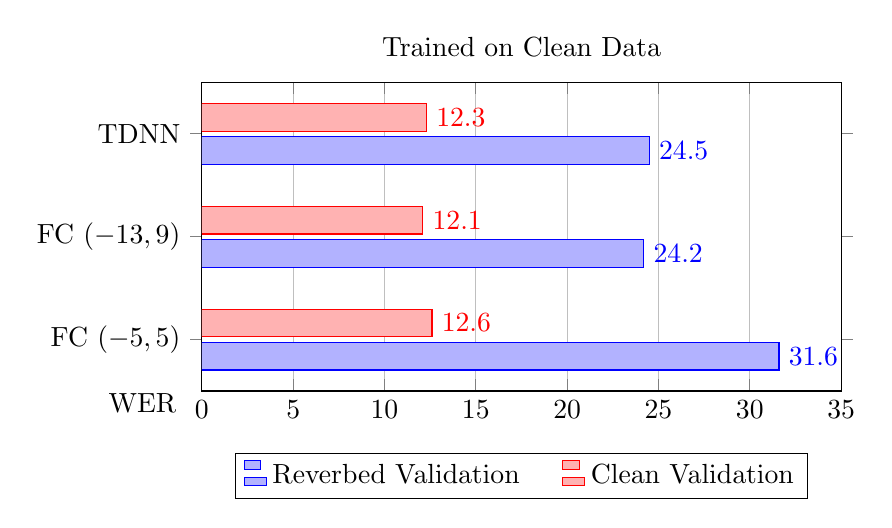
\begin{tikzpicture}
\begin{axis}[
title=Trained on Clean Data,
xbar,xmajorgrids=true,
width=0.8\linewidth,height=5.5cm, enlarge y limits=0.25,
xmin=0,xmax=35,xlabel={WER},xlabel style={
	at={(ticklabel cs:0)},
	anchor=north east,
	yshift=0.56 cm, xshift=-0.2cm
},
symbolic y coords={FC \text{$(-5,5)$}, FC \text{$(-13,9)$}, TDNN},
ytick=data,nodes near coords, nodes near coords align={horizontal},
legend style={at={(0.5,-0.2)},
	anchor=north,legend columns=2}
]
\addplot coordinates {(31.6,FC \text{$(-5,5)$}) (24.2,FC \text{$(-13,9)$}) (24.5,TDNN)};
\addlegendentry{Reverbed Validation \quad \quad}
\addplot coordinates {(12.6,FC \text{$(-5,5)$}) (12.1,FC \text{$(-13,9)$}) (12.3,TDNN)};
\addlegendentry{Clean Validation}
\end{axis}
\end{tikzpicture}
\end{minipage}
\\ \\ \\ 
\begin{minipage}{\linewidth}
\centering
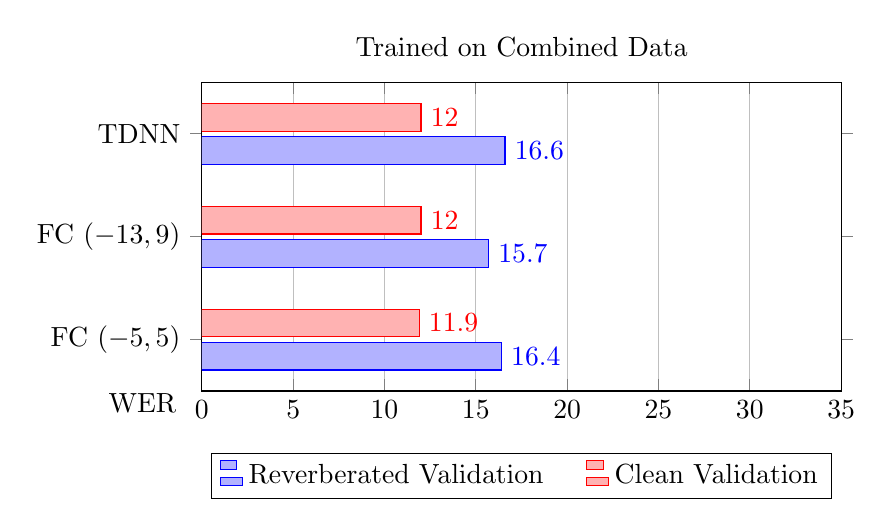
\begin{tikzpicture}
	\begin{axis}[
	title=Trained on Combined Data,
	xbar,xmajorgrids=true,
	width=0.8\linewidth,height=5.5cm, enlarge y limits=0.25,
	xmin=0,xmax=35,xlabel={WER}, xlabel style={
       at={(ticklabel cs:0)},
	   anchor=north east,
	   yshift=0.56 cm, xshift=-0.2cm
	},
	symbolic y coords={FC \text{$(-5,5)$}, FC \text{$(-13,9)$}, TDNN},
	ytick=data,nodes near coords, nodes near coords align={horizontal},
	legend style={at={(0.5,-0.2)},
		anchor=north,legend columns=2}
	]
	\addplot coordinates {(16.4,FC \text{$(-5,5)$}) (15.7,FC \text{$(-13,9)$}) (16.6,TDNN)};
	\addlegendentry{Reverberated Validation \quad \quad}
	\addplot coordinates {(11.9,FC \text{$(-5,5)$}) (12,FC \text{$(-13,9)$}) (12,TDNN)};
	\addlegendentry{Clean Validation}
	\end{axis}
	\end{tikzpicture}
	\captionof{figure}{Word error rate on the clean and reverberated validation dataset for models trained on clean and combined training data, respectively}
	\label{fig:final_validation}
\end{minipage} 
\end{minipage} 
\\ \\ \\
The results of the validation can be seen in figure \ref{fig:final_validation}. For models trained on clean data, the word error rate on the reverberated validation set is high. It can be seen that models with larger input context performed better on unseen reverberated data. On the clean validation set, all models performed similar. \\ \\
For models trained on reverberated data, the performance on the reverberated validation set is similar for all three models. The same holds for clean validation data. The fully connected model with a large input context outperformed the other models on the reverberated validation set by a small margin. All models performed slightly better on clean validation data than their counterpart that was trained on clean data only, where the difference was most significant for the fully connected model with short input context. \\ \\
From this observations we conclude that data augmentation can be sufficient for improving acoustic model performance for reverberated audio. A larger input context can improve the robustness of the acoustic model in some cases. 
\iffalse
TODO: Describe how we generated reverbed data
TODO: Describe how we tested on reverbed data
TODO: Describe final architecture and results

This chapter should summarize and interpret the results. It should give a clear insight
about which methods did decrease the FER and WER on reverbed and unreverbed data, respectivley.
\fi
%% LaTeX2e class for student theses
%% sections/conclusion.tex
%% 
%% Karlsruhe Institute of Technology
%% Institute for Program Structures and Data Organization
%% Chair for Software Design and Quality (SDQ)
%%
%% Dr.-Ing. Erik Burger
%% burger@kit.edu
%%
%% Version 1.3.2, 2017-08-01

\chapter{Conclusion}
\label{ch:Conclusion}
During our evaluation in chapter \ref{ch:results} we found that our TDNN model did not yield a significant improvement over a fully connected model when trained on reverberated data. We also found that a fully connected model with the same input context was capable of slightly outperforming our TDNN model on the reverberated validation set. This results are difficult to generalize to TDNNs as a whole for the following reasons: 
\begin{itemize}
	\item In chapter \ref{ch:tdnn_design}, we tuned our TDNN on clean data, with the assumption that a TDNN model that performs well on clean data also performs well on reverberated data. 
	\item The room impulse response normalization given in \ref{ch:results} might have been too aggressive, thus negating the advantage of TDNNs. In general, it is hard to measure the comprehensibleness of reverberated audio objectively.  
	\item In literature \cite{peddinti2015jhu} \cite{peddinti2015reverberation}, sMBR training criteria are used for TDNN acoustic model training. It might be worth to investigate this training procedure more closely when working with reverberated data.  
\end{itemize}
While the question whether TDNNs or fully connected networks are better for reverberation robust acoustic modeling is still unanswered, we provide several insights that can improve speech recognition systems:
\begin{itemize}
	\item The modified L2 pooling nonlinearity introduced in section \ref{sec:tdnn_nonlin} performed better than L2 pooling combined with normalization.
	\item Augmented data can be used to boost the performance of acoustic models, even when only clean audio is of concern, as shown in chapter \ref{ch:results}.
	\item The calculation of priors from the network output, as shown in section \ref{sec:tdnn_prior}, given a randomly sampled subset of the training data, was shown to outperform priors which were calculated from the training data set. 
	\item We also provided a mathematically sound differentiation of discriminative training criteria for neural networks in section \ref{sec:nn_am}, which is not available in literature in this form.
\end{itemize}
Overall, we were able to show that acoustic models can be made robust against reverberation, if they are trained using reverberated data as well, especially when the input context is large enough. 

%% --------------------
%% |   Bibliography   |
%% --------------------

%% Add entry to the table of contents for the bibliography
\printbibliography[heading=bibintoc]

%% ----------------
%% |   Appendix   |
%% ----------------
\appendix
%% LaTeX2e class for student theses
%% sections/apendix.tex
%% 
%% Karlsruhe Institute of Technology
%% Institute for Program Structures and Data Organization
%% Chair for Software Design and Quality (SDQ)
%%
%% Dr.-Ing. Erik Burger
%% burger@kit.edu
%%
%% Version 1.3.2, 2017-08-01


\chapter{Appendix}
\label{ch:appendix}
\section{Optimal Decoder Parameters}
The following table contains a summary of all decoder parameters we found to be optimal for the experiments in our evaluation. This might be useful for reproducing our results or for further experiments. The table also shows the achieved word error rate on the clean and reverberated development data set. \\ \\ 
\begin{minipage}{\linewidth}
	\centering
	\begin{tabular}{@{\extracolsep{4pt}}lcccclll@{}}
		\toprule
		Model Name      & Training Data & $l_p$ & $l_z$ & $mb$ &  $1/\tau$ & clean WER & rvb WER \\\cmidrule[1pt]{1-1}\cmidrule[1pt]{2-8}
		TDNN $(-13, 9)$ & clean         & -15   & 95    & 6     & 0.9       & 14.9 & 27.6 \\
		FC $(-13, 9)$   & clean         & -10   & 90    & 6     & 0.8       & 15.1 & 28.4 \\
		FC $(-5, 5)$    & clean         & -10   & 90    & 6     & 0.8       & 15.3 & 35.5  \\\cmidrule[1pt]{1-1}\cmidrule[1pt]{2-8}
		TDNN $(-13, 9)$ & clean + rvb   & -5    & 95    & 6     & 0.85      & 14.8 & 20.4 \\
		FC $(-13, 9)$   & clean + rvb   & -10   & 90    & 6     & 0.78      & 14.7 & 19.8 \\
		FC $(-5, 5)$    & clean + rvb   & -10   & 95    & 6     & 1.0       & 14.6 & 20.3\\
		\bottomrule
	\end{tabular}
	\captionof{table}{Optimal decoder parameters and word error rate on clean and reverberated development data set}
	\label{tbl:decoder_params}
\end{minipage} \\ \\
It should be noted that the parameters shown here are implementation specific to the Janus recognition toolkit \cite{finke1997karlsruhe}.

\end{document}
